\documentclass[../Master.tex]{subfiles}
\begin{document}



\[ c_t^+ = \{ x \; | \; x \in U_t^+ \land g(x) \notin s_t \} \]

\[ c_t^- = \{ x : x \in U_t^- \land g(x) \in s_t \} \]

\begin{cor}
    If $g \left[ K_{t-1} \right] \cap s_{t-1} = \emptyset$, then $c_t^+ \cap P^+ \cup c_t^- \cap P^- \neq \emptyset$
\end{cor}

\begin{itemize}
    \item If the action
    application is unsuccessful, ie. if $s=s'$, then at least one of $A$'s
    preconditions were not satisfied by $s$. From this information, however, it
    is unclear which predicates should have been absent from or present in $s$
    for the application to be successful: any ungrounded variant of a predicate
    $p\notin s$ resp. $q\in s$ would cause the failure if part of $P^{+}$ resp.
    $P^{-}$.

    \item When $a$ was successfully applied, ie. when $s\neq s'$, all
    preconditions of $A$ were satisfied, such that $g\left[P^{+}\right]\subseteq
    s$ and $g\left[P^{-}\right]\cap s=\emptyset$. It follows logically that no
    ungrounded version of a predicate $p\in s$ resp. $q\notin s$ can be part of
    $P^{-}$ resp. $P^{+}$, as that would have caused the action to fail.
    However, it is not clear which predicates in $s$ and $s^{C}$ satisfied the
    preconditions, as some of them may have been redundant.
\end{itemize}
Thus,     only when action applications are successful can predicates be
disproven to     be preconditions, but no predicate can be proven to be a
precondition based     solely on a state transition.

Consider the addition of prior knowledge $\left(K^{+},K^{-},U^{+},U^{-}\right)$,
and assume that $s$ does not violate any precondition that is already known to
be true (ie. $g\left[K^{+}\right]\subseteq s$ and $g\left[K^{-}\right]\cap
s=\emptyset$). Then, in the case of action failure, any violated precondition
$p$ must exist in either $U^{+}$ or $U^{-}$. The ungrounded predicates that
would individually cause the failure if they were present in $P^{+}$ (resp.
$P^{-}$) are denoted $c^{+}$ (resp. $c^{-}$), and are determined as follows:

\[ c^{+}=U^{+}\setminus\bigcup ug\left[s\right] \] \[ c^{-}=U^{-}\cap\bigcup
ug\left[s\right] \]

For any \emph{candidate set} $c=\left(c^{+},c^{-}\right)$ constructed in this
manner, it holds that at least one of the candidates is a precondition of $A$,
ie. \begin{equation} c^{+}\cap P^{+}\neq\emptyset\lor c^{-}\cap
P^{-}\neq\emptyset\label{eq:cP} \end{equation}

\begin{cor} \label{candThe}Trivially, if (\ref{eq:cP}) holds and $c^{+}=\left\{
p\right\} \land c^{-}=\emptyset$, then $p\in P^{+}$. Conversely, if
$c^{+}=\emptyset\land c^{-}=\{q\}$, then $q\in P^{-}$. \end{cor} Notably, if
several members of $c^{+}\cup c^{-}$ are preconditions of $A$, it can never be
recuced to a singleton set, and no information can be gained from it.

If, in a later state transition for the same action schema $A$, a predicate $p$
is proven to be absent from $P^{\pm}$, then it is no longer a valid candidate,
and can be removed from $c^{\pm}$ while maintaining the validity of
(\ref{eq:cP}).

If, however, a predicate $q\in c^{+}\cup c^{-}$ is proven to be a precondition,
then removal of $q$ from $c$ might violate (\ref{eq:cP}). If $q$ is retained in
$c$, then one of the following cases apply: \begin{itemize} \item
$\left(c^{+}\cap P^{+}\right)\cup\left(c^{-}\cap P^{-}\right)=\{q\}$, ie. $q$ is
the only predicate in $c$ that is a precondition. Then $c$ could eventually be
reduced to the singleton set $\{q\}$, which does not produce any new knowledge,
since $q$ is already known to be a precondition. \item $\left|\left(c^{+}\cap
P^{+}\right)\cup\left(c^{-}\cap P^{-}\right)\right|>1$, ie. more than two
predicates in $c$ are preconditions of $A$. As mentioned above, $c$ can never be
reduced to the singleton set, and no knowledge can be gained from it.
\end{itemize} In both cases, retaining the set $c$ as it is will not provide any
new knowledge. Thus, a candidate set can be discarded when one of its predicates
are proven to be present in $P^{\pm}$.

We can now define a precondition hypothesis as follows: \begin{defn} A
precondition hypothesis $H_{P}$ for an action schema $A$ is a five-tuple
$\left(K^{+},K^{-},U^{+},U^{-},C\right)$, where $C$ is a set of candidate sets.
\end{defn} Whenever new knowledge about a predicate is obtained, $C$ is updated
using the following rules, ensuring that (\ref{eq:cP}) holds for all candidate
sets in $C$:
\begin{enumerate}
    \item If a predicate $p$ is proven to be absent
from $P^{+}$, it is removed from all positive parts of candidate sets in $C$
(similarly for $P^{-}$ and negative parts):
    \[ C_t = \left\{ \left(x^{+}\cap
U^{+},x^{-}\cap U^{-}\right):\left(x^{+},x^{-}\right)\in C_{t-1} \right\} \]

    \item If a predicate $p$ is proven to be present in $P^{+}$ or $P^{-}$, any candidate set containing $p$ is removed from $C$:
    \[ C_t = \left\{ \left( x^{+},x^{-} \right) : \left(x^{+},x^{-}\right)\in C_{t-1} \land\left(x^{+}\cap
K^{+}\neq\emptyset\lor x^{-}\cap K^{-}\neq\emptyset\right)\right\} \]

\end{enumerate} Given a state transition $\left(s,a,s'\right)$ and a
precondition hypothesis $H_{P}$, we can now produce an updated hypothesis by the
following two cases: \begin{description} \item [{Action\ failure:}] The
candidate set $c$ is determined as described above. If $c$ is the singleton set,
the contained predicate is added to $K^{\pm}$ and removed from $U^{\pm}$, and
$C$ is updated using rules 1 and 2. Otherwise, $c$ is added to $C$. \item
[{Action\ success:}] Since all preconditions are satisfied, all ungrounded
versions of predicates in $s$ are disproven to be negative predicates, and all
ungrounded versions of predicates $q\notin s$ are disproven to be positive
predicates, formally: \[ U^{+\prime}=U^{+}\cap\bigcup u\left(s\right) \] \[
U^{-\prime}=U^{-}\setminus\bigcup u\left(s\right) \] Now, $C$ can be updated
using rule 1, and theorem \ref{candThe} can be used on each candidate set in $C$
to add singleton sets to $K^{+}$ and $K^{-}$: \[ K^{\pm\prime}=\left\{
x^{\pm}:\left(x^{+},x^{-}\right)\in
C^{\prime}\land\left|x^{\pm}\right|=1\land\left|x^{+}\right|+\left|x^{-}\right|=1\right\}
\cup K^{\pm} \] As this may prove the presence of predicates in $P^{\pm}$, $C$
must be updated using rule 2. \end{description}

\subsection{Undiscoverable preconditions}

To see this machinery in action, we once again apply it to the sokoban domain.

\begin{figure}
    \centering
    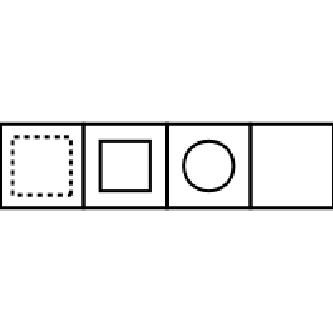
\includegraphics[scale=0.7]{../Graphics/sokoSmall}
    \caption{\label{fig:sokoSmall} Sokoban state with only one applicable \texttt{move-h} action. The tiles are named $t_1 \dots t_4$, from left to right.}
\end{figure}


\begin{equation}
U_0^+ = U_0^- =
\left\{
    \begin{gathered}
        \texttt{sokobanAt}(to), \texttt{sokobanAt}(from), \\
        \texttt{clear}(to), \texttt{clear}(from), \\
        \texttt{goal}(to), \texttt{goal}(from), \\
        \texttt{vAdj}(from), \texttt{vAdj}(to), \\
        \texttt{hAdj}(from), \texttt{hAdj}(to), \\
        \texttt{at}(from, to), \texttt{at}(to, from)
    \end{gathered}
\right\}
\end{equation}

If the agent decides that to move one tile to the right, and executes the \texttt{move-h}$(t_3, t_2)$ action, it will discover that the new state is exactly the same as the old, and that the action therefore must have failed. The ungrounded predicates that could have caused the failure are then the following:

\begin{align}
(c_1^+, c_1^-) =
\left(
    \left\{
        \begin{gathered}
            \texttt{sokobanAt}(to), \\
            \texttt{clear}(to), \texttt{clear}(from), \\
            \texttt{goal}(to), \texttt{goal}(from), \\
            \texttt{vAdj}(from), \texttt{vAdj}(to), \\
            \texttt{at}(from, to), \texttt{at}(to, from)
        \end{gathered}
    \right\}
    ,
    \left\{
        \begin{gathered}
            \texttt{sokobanAt}(from), \\
            \texttt{hAdj}(from), \texttt{hAdj}(to)
        \end{gathered}
    \right\}
\right)
\end{align}

If --- in the next simulation step --- the agent tries to move right using the action \texttt{move-h}$(t_3, t_4)$, the resulting state will be different, meaning that the action application was successful.

% sokoban successfully executes action move-h(t3, t4)

\[
U_2^+ = \{ \texttt{sokobanAt}(from), \texttt{clear}(to), \texttt{hAdj}(from, to), \texttt{hAdj}(to, from) \}
\]
\[
U_2^- = \{ \texttt{sokobanAt}(to), \texttt{clear}(from), \texttt{vAdj}(from, to), \texttt{vAdj}(to, from), \texttt{at}(to, from), \texttt{at}(from, to) \}
\]

\[
(c_1^+ \cap U_2^+, c_1^- \cap U_2^-) = ( \{ \texttt{clear}(to) \}, \; \emptyset )
\]

\end{document}
